\documentclass{article}
\usepackage[utf8]{inputenc}
\usepackage{tikz}
\usetikzlibrary{shapes, arrows.meta, positioning, calc}
\usepackage{geometry}
\usepackage{amsmath}
\usepackage{array}
\usepackage{enumerate}
\usepackage{fancyvrb} % For displaying code/commands

\geometry{
    a4paper,
    margin=1in,
}

\begin{document}

\title{Cybersecurity (CSCI 2413): Mid-Term Review Study Guide}
\author{Based on Course Slides}
\date{\today}
\maketitle

\section{Open-Source Intelligence (OSINT)}

\subsection{Definition and Scope}

\begin{itemize}
    \item \textbf{OSINT (Open-Source Intelligence)}: Collecting and analyzing publicly available information to gather insight and information on a target.
    \item The information gathered can come from various sources including media (interviews, CT, leaflicts/books), reports (governments, NGOs, journalists), deliverables (websites, forums, social media, videos/audio recordings), and academic research.
\end{itemize}

\subsection{OSINT Workflow/Steps}
\begin{enumerate}
    \item \textbf{Planning and Direction}: Establish clear objectives by defining what information is needed and why.
    \item \textbf{Collection}: Data gathering from public sources, social media, public records. Uses manual and automated methods.
    \item \textbf{Processing and Organization}: Filter raw data for relevance and remove duplicates (often a manual process).
    \item \textbf{Analysis and Correlation}: Identify patterns, relationships, and trends. Corroborate findings with multiple sources to ensure accuracy.
    \item \textbf{Dissemination}: Report the final findings in a structured way (Report, Briefing) to relevant stakeholders.
\end{enumerate}

\subsection{OSINT Targets}
\begin{itemize}
    \item Individuals
    \item Organizations and Businesses
    \item Critical Infrastructure
    \item Cybersecurity and Threat Intelligence
    \item Governments and Nations
    \item Public Health
\end{itemize}

\subsection{Sock Puppet and Related Concepts}
\begin{itemize}
    \item \textbf{Sock Puppet}: A covert account that is not related to your identity.
    \item Used to protect true identity when performing \textbf{SOCMINT} (Social Media Intelligence).
    \item For investigations/pentests, this should be done from a \textbf{Virtual Machine (VM)} using a \textbf{VPN} (Virtual Private Network).
\end{itemize}

\section{Cryptography Basics}

\subsection{Encryption and Decryption}
\begin{itemize}
    \item \textbf{Encryption}: Algorithm scrambles plain text. Sender and receiver agree on the algorithm. Message is difficult to re-create without the protocol.
    \item \textbf{Decryption}: Reversal of the scrambling protocol to make the message comprehensible.
\end{itemize}

\subsubsection{Symmetric Encryption Flow Diagram}

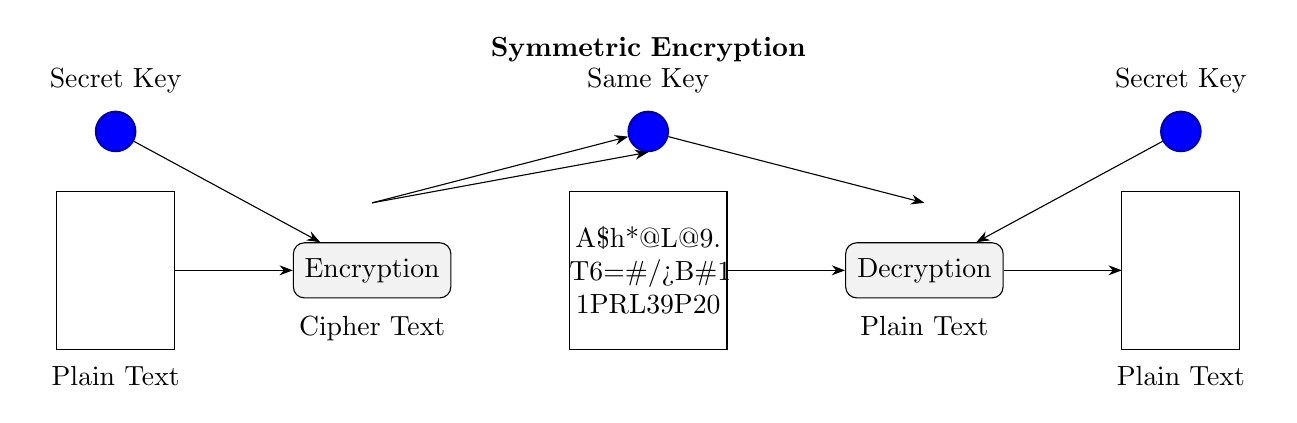
\begin{tikzpicture}[
    >=Stealth,
    file/.style={draw, minimum width=1.5cm, minimum height=2cm, fill=white, inner sep=0pt, outer sep=0pt},
    key/.style={draw, color=blue!70!black, minimum size=0.5cm, thick, path picture={
        \node at (path picture bounding box.center) {\bfseries \color{blue!70!black} \rotatebox{10}{\checkmark}};
        }, circle, fill=blue!10},
    process/.style={draw, rectangle, rounded corners, minimum height=0.7cm, align=center},
    textnode/.style={align=center, text width=2cm},
    ]

    \tikzset{
        keypic/.pic={
            \draw[fill=gray!30, thick] (0, 0) -- ++(0.1, 0.5) arc (90:-90:0.1) -- ++(-0.1, -0.5) -- cycle;
            \draw[fill=gray!30, thick] (0.1, 0.5) arc (90:270:0.1) -- (0.1, 0.5);
            \draw[fill=white, thick] (0.2, 0.4) circle (0.1);
            \draw[fill=white, thick] (0.2, 0.2) circle (0.1);
            \draw[fill=white, thick] (0.2, 0.0) circle (0.1);
        }
    }

    \node (P1) [file] {};
    \node (T1) [textnode, below=0.1cm of P1] {Plain Text};
    
    \node (K1) [key, above=0.5cm of P1, fill=blue] {};
    \node (L1) [above=0.1cm of K1] {Secret Key};

    \node (E) [process, right=1.5cm of P1, minimum width=2cm, fill=black!5] {Encryption};
    \node (T2) [textnode, below=0.1cm of E] {Cipher Text};
    
    \node (C) [file, right=1.5cm of E, minimum width=2cm] {};
    \node (T3) [text width=2cm, align=center] at (C) {A\$h*@L@9. \\ T6=\#/>B\#1 \\ 1PRL39P20};

    \node (K2) [key, above=0.5cm of C, fill=blue] {};
    \node (L2) [above=0.1cm of K2] {Same Key};

    \node (D) [process, right=1.5cm of C, minimum width=2cm, fill=black!5] {Decryption};
    \node (T4) [textnode, below=0.1cm of D] {Plain Text};

    \node (P2) [file, right=1.5cm of D] {};
    \node (T5) [textnode, below=0.1cm of P2] {Plain Text};
    
    \node (K3) [key, above=0.5cm of P2, fill=blue] {};
    \node (L3) [above=0.1cm of K3] {Secret Key};
    
    \draw[->] (P1) -- (E);
    \draw[->] (C) -- (D);
    \draw[->] (D) -- (P2);
    
    \draw[->] (K1) -- (E);
    \draw[->] (K3) -- (D);
    
    \draw[->] ([yshift=0.5cm]E.north) -- ([yshift=0.5cm]C.north); % Connection above the cipher text node
    \draw[->] ([yshift=0.5cm]E.north) -- (K2);
    \draw[->] (K2) -- ([yshift=0.5cm]D.north);
    
    \node at ($(K1)!0.5!(K3)$) [above=0.5cm of K2, text width=6cm, align=center] {\textbf{Symmetric Encryption}};
\end{tikzpicture}

\subsection{Types of Ciphers}
\begin{itemize}
    \item \textbf{Transposition}: Rearranging each letter with a different letter (e.g., Rail Fence cipher).
    \item \textbf{Substitution}: Replaces each letter with a different letter (e.g., Caesar, Vigenere).
    \begin{itemize}
        \item Two types of substitution:
        \begin{enumerate}
            \item \textbf{Single/Symmetric Key Encryption}
            \begin{itemize}
                \item Stream
                \item Block
            \end{itemize}
            \item \textbf{Public/Asymmetric Key Encryption}
        \end{enumerate}
    \end{itemize}
\end{itemize}

\subsection{Transposition Cipher Example: Rail Fence}
Message: ``Defend the east wall'' with a key of 3.

\begin{center}
\begin{tabular}{|>{\centering\arraybackslash}p{0.5cm}|*{14}{>{\centering\arraybackslash}p{0.5cm}|}}
\hline
D & & N & & E & & T & & L & & E & & D & \\
\hline
& E & & E & & D & & H & & E & & S & & W & \\
\hline
& & L & & X & & F & & T & & A & & A & X \\
\hline
\end{tabular}
\end{center}
The ciphertext is read off row by row to get: \textbf{DNETLEEDHESWLXFTAAX}.

\subsection{Substitution Cipher Example: Caesar Cipher}
\begin{itemize}
    \item \textbf{Caesar Cipher}: A shift cipher.
    \item Example Key $+2$:
    \begin{itemize}
        \item Cleartext: HELLO WORLD
        \item Alphabet: A B C D E F G H I J K L M N O P Q R S T U V W X Y Z
        \item Shifted: C D E F G H I J K L M N O P Q R S T U V W X Y Z A B
        \item Cipher Text: \textbf{JGNNQ YQTNF}
    \end{itemize}
    \item \textbf{Frequency distribution} will crack the simple Caesar cipher.
\end{itemize}

\subsection{Vigenere Cipher}
\begin{itemize}
    \item Uses a plaintext, a key, and a keystream (the key repeated) applied via the Vigenere square (or tabula recta).
    \item Example: Plaintext: ATTACKATDAWN, Key: LEMON, Keystream: LEMONLEMONLE, Ciphertext: \textbf{LXFOPVEFRNHR}.
\end{itemize}

\subsection{Historical Cryptography}
\begin{itemize}
    \item \textbf{Charles Babbage}: Broke the Vigenere Cipher in 1854.
    \item \textbf{Arthur Scherbius}: Created the \textbf{Enigma} machine in 1918. Key components included Rotors, Lampboard, Keyboard, and Plugboard.
    \item \textbf{Alan Turing}: Created the first \textbf{Bombe} in the 1940s, which helped crack the Enigma codes.
    \item \textbf{Turing Test}: An interviewer asks the same question of a computer and a human to determine if you are talking to a computer or human.
\end{itemize}

\subsubsection{Alan Turing – 6 Primitives (Turing Machine)}
The 6 basic operations considered a software language:
\begin{itemize}
    \item \textbf{Right}: Move the Machine’s head to the right of the current square.
    \item \textbf{Left}: Move the Machine’s head to the left of the current square.
    \item \textbf{Print}: Print a symbol on the current square.
    \item \textbf{Scan}: Identify any symbols on the current square.
    \item \textbf{Erase}: Erase any symbols presented on the current square.
    \item \textbf{Nothing/Halt}: Do nothing.
\end{itemize}

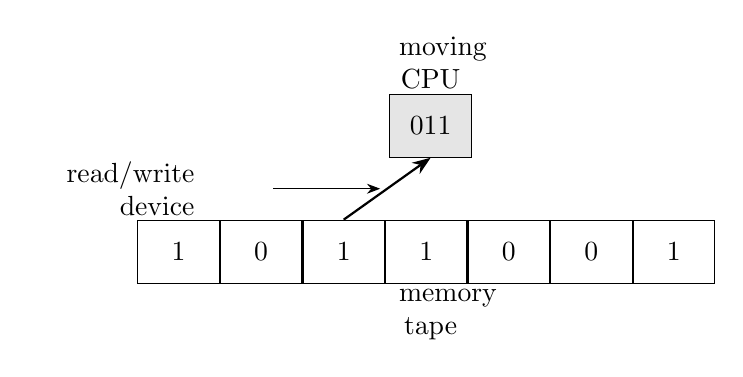
\begin{tikzpicture}[>=Stealth, scale=0.8, every node/.style={draw, minimum size=0.8cm, text width=0.8cm, align=center}]
    \node (CPU) at (0, 3) [draw=none, minimum size=0cm] {moving CPU};
    \node (Head) at (0, 2) [fill=gray!20] {011};
    
    \node (T1) at (-4, 0) {1};
    \node (T2) [right=0pt of T1] {0};
    \node (T3) [right=0pt of T2] {1};
    \node (T4) [right=0pt of T3] {1};
    \node (T5) [right=0pt of T4] {0};
    \node (T6) [right=0pt of T5] {0};
    \node (T7) [right=0pt of T6] {1};
    
    \draw[->, thick] (T3.north) -- (Head.south);
    
    \node at (-5, 1) [draw=none, text width=2cm, align=right] {read/write device};
    \draw[->] (-2.5, 1) -- (-0.8, 1);
    
    \node at (0, -1) [draw=none, minimum size=0cm] {memory tape};
\end{tikzpicture}

\section{Key Exchange and Public Key Infrastructure}

\subsection{Diffie Hellman Key Exchange (DHKE)}
DHKE allows two parties to establish a shared secret key over an insecure communication channel.

\subsubsection{Diffie Hellman Example (Numbers)}
The protocol relies on modular exponentiation: $A = g^a \pmod{p}$ and $B = g^b \pmod{p}$. The shared secret is $S = (B^a) \pmod{p} = (A^b) \pmod{p}$.

\begin{center}
\begin{tabular}{|m{2.5cm}|m{1cm}|m{2.5cm}|m{1cm}|m{2.5cm}|m{1cm}|}
\hline
\multicolumn{2}{|c|}{\textbf{Alice}} & \multicolumn{2}{|c|}{\textbf{Bob}} & \multicolumn{2}{|c|}{\textbf{Eve}} \\
\hline
\textbf{Known} & \textbf{UN} & \textbf{Known} & \textbf{UN} & \textbf{Known} & \textbf{UN} \\
\hline
$p=23$ & & $p=23$ & & $p=23$ & \\
\hline
$g=5$ & & $g=5$ & & $g=5$ & \\
\hline
$a=6$ & $b$ & $b=15$ & $a$ & & $a, b$ \\
\hline
$A=5^a \pmod{23}$ & & $B = 5^b \pmod{23}$ & & & \\
\hline
$A=5^6 \pmod{23} = 8$ & & $B=5^{15} \pmod{23} = 19$ & & & \\
\hline
$B=19$ & & $A=8$ & & $A=8, B=19$ & \\
\hline
$S=B^a \pmod{23}$ & & $S=A^b \pmod{23}$ & & & \\
\hline
$S=19^6 \pmod{23} = 2$ & & $S=8^{15} \pmod{23} = 2$ & & & $S$ \\
\hline
\end{tabular}
\end{center}

\subsubsection{Diffie Hellman Example (Colors)}
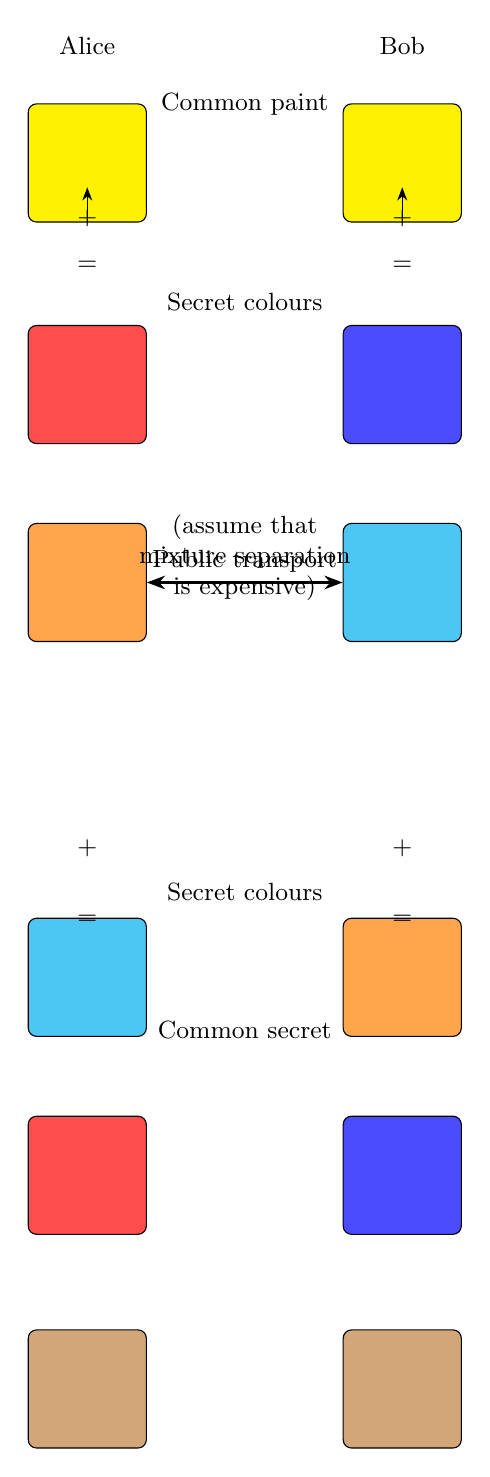
\begin{tikzpicture}[
    >=Stealth,
    jar/.style={draw, minimum width=1.5cm, minimum height=1.5cm, trapezium, trapezium angle=70, shape border rotate=180, fill=white, inner sep=0pt},
    colorjar/.style={draw, minimum width=1.5cm, minimum height=1.5cm, fill, inner sep=0pt, rounded corners=3pt},
    font=\small
]

% Define color mixing nodes (using rounded rectangles for simplification)
\node (A) at (0, 0) {Alice};
\node (B) at (4, 0) {Bob};

% Common Paint (Yellow)
\node (AC1) [colorjar, fill=yellow, below=0.5cm of A] {};
\node (BC1) [colorjar, fill=yellow, below=0.5cm of B] {};
\node at (2, -0.75) {Common paint};

\draw[->] (AC1) -- (0, -1.8);
\draw[->] (BC1) -- (4, -1.8);

% Secret Colors (Red and Blue)
\node (AS1) [colorjar, fill=red!70, below=1.3cm of AC1] {};
\node (BS1) [colorjar, fill=blue!70, below=1.3cm of BC1] {};
\node at (2, -3.25) {Secret colours};

\node (Mix1) at (0, -2.5) {};
\node (Mix2) at (4, -2.5) {};

\draw (0, -2.2) node {$+$};
\draw (4, -2.2) node {$+$};
\draw (0, -2.8) node {=};
\draw (4, -2.8) node {=};

% Public Mixed Paint (Orange and Light Blue)
\node (APub) [colorjar, fill=orange!70, below=1cm of AS1] {};
\node (BPuB) [colorjar, fill=cyan!70, below=1cm of BS1] {};

% Exchange path
\draw[<->, thick] (APub.east) -- node[above, align=center] {Public transport} (BPuB.west);
\node at (2, -6.5) [text width=3cm, align=center] {(assume that mixture separation is expensive)};

% Alice receives Bob's public mix, Bob receives Alice's public mix
\node (AS2) [colorjar, fill=cyan!70, below=3.5cm of APub] {};
\node (BS2) [colorjar, fill=orange!70, below=3.5cm of BPuB] {};

% Re-add secret colors
\node (AS3) [colorjar, fill=red!70, below=1cm of AS2] {};
\node (BS3) [colorjar, fill=blue!70, below=1cm of BS2] {};
\node at (2, -10.75) {Secret colours};

\draw (0, -10.2) node {$+$};
\draw (4, -10.2) node {$+$};
\draw (0, -11.1) node {=};
\draw (4, -11.1) node {=};

% Common Secret (Brown)
\node (AFin) [colorjar, fill=brown!70, below=1.2cm of AS3] {};
\node (BFin) [colorjar, fill=brown!70, below=1.2cm of BS3] {};
\node at (2, -12.5) {Common secret};

\end{tikzpicture}

\subsection{Asymmetric Encryption (Public Key Cryptography)}
\begin{itemize}
    \item Uses two different keys: a \textbf{Public Key} (shared) and a \textbf{Secret Key} (kept private).
\end{itemize}

\subsubsection{Asymmetric Encryption Flow Diagram}
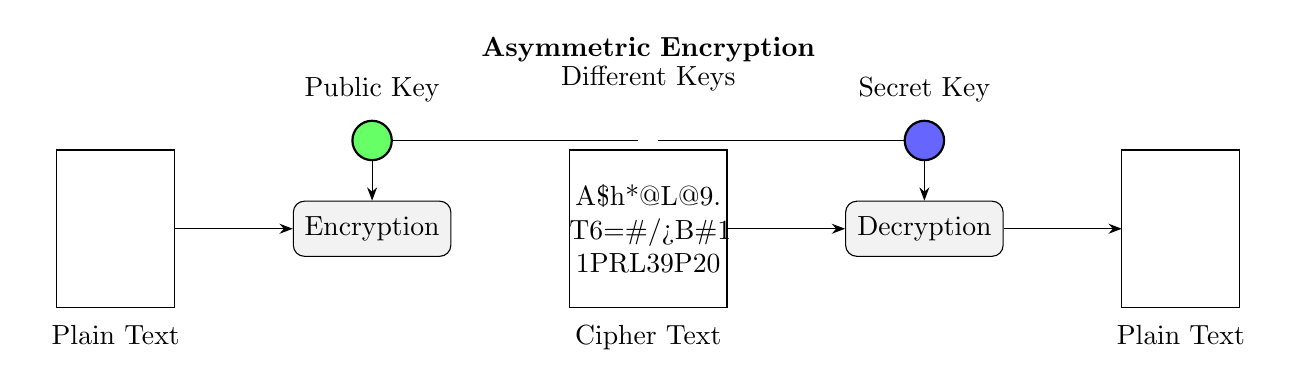
\begin{tikzpicture}[
    >=Stealth,
    file/.style={draw, minimum width=1.5cm, minimum height=2cm, fill=white, inner sep=0pt, outer sep=0pt},
    key/.style={circle, draw, minimum size=0.5cm, thick},
    process/.style={draw, rectangle, rounded corners, minimum height=0.7cm, align=center},
    textnode/.style={align=center, text width=2cm},
    ]

    \node (P1) [file] {};
    \node (T1) [textnode, below=0.1cm of P1] {Plain Text};
    
    \node (E) [process, right=1.5cm of P1, minimum width=2cm, fill=black!5] {Encryption};
    \node (C) [file, right=1.5cm of E, minimum width=2cm] {};
    \node (T3) [text width=2cm, align=center] at (C) {A\$h*@L@9. \\ T6=\#/>B\#1 \\ 1PRL39P20};
    \node (T2) [textnode, below=0.1cm of C] {Cipher Text};
    
    \node (D) [process, right=1.5cm of C, minimum width=2cm, fill=black!5] {Decryption};
    \node (P2) [file, right=1.5cm of D] {};
    \node (T4) [textnode, below=0.1cm of P2] {Plain Text};

    % Keys
    \node (PK) [key, fill=green!60, above=0.5cm of E] {};
    \node (SK) [key, fill=blue!60, above=0.5cm of D] {};
    
    \node (KeyLine) at ($(PK)!0.5!(SK)$) {};
    \draw (PK) -- (KeyLine);
    \draw (SK) -- (KeyLine);
    
    \node (PKL) [above=0.1cm of PK] {Public Key};
    \node (SKL) [above=0.1cm of SK] {Secret Key};
    
    \node at (KeyLine) [above=0.5cm, text width=4cm, align=center] {Different Keys};

    \draw[->] (P1) -- (E);
    \draw[->] (C) -- (D);
    \draw[->] (D) -- (P2);
    
    \draw[->] (PK) -- (E);
    \draw[->] (SK) -- (D);

    \node at ($(P1)!0.5!(P2)$) [above=2cm, text width=8cm, align=center] {\textbf{Asymmetric Encryption}};
\end{tikzpicture}

\subsection{Certificate Authorities and PKI}
\begin{itemize}
    \item \textbf{Certificate Authorities (CA)}: Primary role is to digitally sign and publish the public key of a given user.
    \item \textbf{Registration Authority (RA)}: Often handles verification prior to certificates being issued.
    \item \textbf{Public Key Infrastructure (PKI)}: An arrangement that binds public keys with respective user identities by means of a CA.
\end{itemize}

\section{Hashing and Data Integrity}

\subsection{Hashing}
\begin{itemize}
    \item \textbf{Hashing}: Takes a variable-size input and returns a fixed-size string (the \textbf{hash value}).
    \item Hashing is \textbf{one-way}; you cannot un-hash something.
    \item Hashing is how Windows stores passwords.
\end{itemize}

\subsubsection{Salting}
\begin{itemize}
    \item \textbf{Salt}: Refers to random bits that are used as one of the inputs to the hash.
    \item Salting uses a randomly generated string used with the hash so each hashed password will be unique, even if the passwords are the same.
    \item Complicates dictionary and rainbow table attacks.
\end{itemize}

\begin{center}
\textbf{Salting Example}
\end{center}
\begin{tabular}{|m{2cm}||m{2cm}|m{2cm}|m{2cm}|m{2cm}|}
\hline
\textbf{Field} & \multicolumn{2}{c|}{User 1 (No Salt)} & \multicolumn{2}{c|}{User 2 (Salted)} \\
\hline
Password & p4s5w3rdz & p4s5w3rdz & p4s5w3rdz & p4s5w3rdz \\
\hline
Salt & -- & -- & et52ed & ye5sf8 \\
\hline
Hash & f4c31aa & f4c31aa & 1vn49sa & z32i6t0 \\
\hline
\end{tabular}

\subsection{Hashing Methods}
\begin{itemize}
    \item \textbf{Secure Hash Algorithm (SHA)}: Most widely used (SHA-1, SHA-2, SHA-3, SHA-256, SHA-512).
    \item \textbf{MD5}: Not collision resistant.
    \item \textbf{RACE Integrity Primitives Evaluation Message Digest (RIPEMD)}.
\end{itemize}

\subsection{Steganography}
\begin{itemize}
    \item \textbf{Steganography}: The art and science of writing hidden messages in such a way that nobody other than the sender and intended recipient suspects the existence of the message.
    \item Message is often hidden in some other file (e.g., digital picture or audio file).
    \item Messages do not attract attention to themselves.
\end{itemize}

\section{Social Engineering}

\subsection{Introduction and Techniques}
\begin{itemize}
    \item \textbf{Social engineering}: The psychological manipulation of people into performing actions or divulging confidential information.
    \item Key Attack Techniques:
    \begin{enumerate}
        \item \textbf{Commitment}
        \item \textbf{Authority}
        \item \textbf{Reciprocation}
        \item \textbf{Reverse Engineering}
        \item \textbf{Likening}
        \item \textbf{Scarcity}
    \end{enumerate}
\end{itemize}

\subsection{Detailed Techniques}
\begin{itemize}
    \item \textbf{Commitment}: Occurs when the attacker tricks the victim into making a promise which they feel obligated to keep.
    \begin{itemize}
        \item \textbf{Conformity}: A special type of commitment leveraging an implied commitment made by society (e.g., leaving a tip).
    \end{itemize}
    \item \textbf{Authority}: The process of an attacker assuming a role of authority which they do not possess. Types:
    \begin{itemize}
        \item \textbf{Impersonation}: Pretending to be someone they are not.
        \item \textbf{Diffusion of Responsibility}: Manipulating decision-making from individual to collective.
        \item \textbf{Reciprocation}: Giving the victim a gift, leading the victim to feel social pressure to return the favor.
    \end{itemize}
    \item \textbf{Reverse Social Engineering}: An attack where the aggressor tricks the victim into asking him for assistance. Steps:
    \begin{enumerate}
        \item \textbf{Sabotage}: Attacker creates a problem compelling the victim to action.
        \item \textbf{Advertise}: Attacker advertises willingness/ability to solve the problem.
        \item \textbf{Assist}: Attacker requests assistance from the victim to solve the problem (e.g., requesting passwords).
    \end{enumerate}
    \item \textbf{Likening}: An attacker behaves in a way to appear similar to a member of a trusted group (Political, Religious, Hobbies) to gain confidence.
    \item \textbf{Scarcity}: Attacker introduces the perception of scarcity of an item that is highly valued.
    \begin{itemize}
        \item \textbf{Rushing}: Putting severe time constraints on a decision.
    \end{itemize}
\end{itemize}

\subsection{Defenses}
The most effective defense against social engineering attacks is \textbf{EDUCATION}.
\begin{itemize}
    \item \textbf{Training}: Repeat often.
    \item \textbf{Reaction}: Recognize the attack and move to a more alert state.
    \item \textbf{Inoculation}: Making attack resistance a normal part of the work experience.
\end{itemize}

\subsection{Physical Security Attacks}
\begin{itemize}
    \item \textbf{Tailgating}: Seeking entry to a restricted area by walking in after someone else has opened the door.
    \item \textbf{Shoulder Surfing}: Looking over someone's shoulder to see them type passwords or read confidential documents.
    \item \textbf{Leaving Computer Unlocked}: (TRUST NO ONE).
\end{itemize}

\section{Information Theft and Phishing}

\subsection{Personally Identifiable Information (PII)}
PII sought by attackers includes:
\begin{itemize}
    \item \textbf{Name}: Full Name, maiden name, mother’s maiden name.
    \item \textbf{Personal identification numbers}: Social Security Number (SSN), Passport Number, Drivers License Number, Taxpayer ID.
    \item \textbf{Personal Address}: Street address, city, state, zip.
    \item \textbf{Personal Phone \#/Email}.
    \item \textbf{Personal Characteristics}: Photograph, fingerprints, handwriting.
    \item \textbf{Biometric data}: Retina scans, voice signatures or facial geometry.
    \item \textbf{Financial Data}: Bank accounts, Credit cards, Tax records.
\end{itemize}
Other Shared PII: Date of Birth, Place of Birth, Business Phone/Email/Address, Race, Religion, Employment/Medical/Education/Financial Information.

\subsection{Phishing Attacks}
\begin{itemize}
    \item \textbf{Phishing}: The fraudulent attempt to obtain sensitive information (usernames, passwords, bank account info, etc.).
    \item \textbf{Spear Phishing}: Directed at specific individuals or companies.
    \item \textbf{Whaling}: Targets a specific individual, usually a senior executive (e.g., Jeff Bezos).
    \item \textbf{Vishing}: Voice call phishing.
    \item \textbf{Smishing}: SMS/Text Message phishing.
\end{itemize}

\subsection{Regulation}
\begin{itemize}
    \item \textbf{HIPAA (Health Insurance Portability and Accountability Act)} of 1996: Designed to protect the privacy and security of certain health information.
\end{itemize}

\section{Authentication and Password Attacks}

\subsection{Multi-factor Authentication (MFA)}
\begin{tikzpicture}[
    >=Stealth,
    node distance=1.5cm,
    step/.style={rectangle, draw, rounded corners, minimum height=1cm, text width=2cm, align=center},
    access/.style={circle, draw, very thick, minimum size=2cm, text width=1.5cm, align=center, fill=green!10},
    phone/.style={draw, rectangle, minimum width=1.5cm, minimum height=3cm, rounded corners=5pt},
    comp/.style={draw, rectangle, minimum width=2.5cm, minimum height=1.5cm, rounded corners=3pt},
    title/.style={text width=6cm, align=center, font=\Large\bfseries}
]

\node (Title) at (0, 3.5) [draw=none] {Multi-factor authentication};

% Step 1: Password
\node (S1) [step, text width=3cm] at (-4, 2.5) {Step 1 \\ password};
\node (Computer) [comp, below=0.5cm of S1] {};
\node (Screen) [rectangle, fill=white, draw=gray, minimum width=1.5cm, minimum height=0.7cm] at (-4, 2) {};

% Step 2: Proof
\node (S2) [step] at (0, 2.5) {Step 2 \\ proof};
\node (Phone) [phone, below=0.5cm of S2] {};
\node (PScr) [rectangle, fill=white, draw=gray, minimum width=1cm, minimum height=1.5cm] at (0, 1.85) {};
\node at (0, 1.6) [draw=none, font=\small] {Trust?};
\node (Yes) [draw, rectangle, fill=green!30, font=\tiny] at (-0.3, 1.3) {Yes};
\node (No) [draw, rectangle, fill=red!30, font=\tiny] at (0.3, 1.3) {No};

% Step 3: Access
\node (S3) [step] at (4, 2.5) {Step 3 \\ access};
\node (Access) [access, below=0.5cm of S3] {Access \\ Granted};

% Arrows
\draw[->, dashed] (Computer.east) -- ($(Computer.east)!0.5!(Phone.west)$);
\draw[->, dashed] ($(Computer.east)!0.5!(Phone.west)$) -- (Phone.west);
\draw[->, dashed] (Phone.east) -- ($(Phone.east)!0.5!(Access.west)$);
\draw[->, dashed] ($(Phone.east)!0.5!(Access.west)$) -- (Access.west);

\end{tikzpicture}

\subsection{Password Attacks}
\begin{itemize}
    \item \textbf{Dictionary Attack}: A type of brute-force cyberattack where an attacker uses pre-compiled lists of common passwords, keyboard patterns, and leaked credentials to break into an account.
    \item \textbf{Rule-based attack}: Makes modifications to dictionary words (e.g., replacing ``a'' with ``@'') following password patterns.
    \item \textbf{Mask attack}: An optimized brute-force attack that reduces the search space by exploiting known information about the password format or length.
\end{itemize}

\section{Networking Fundamentals}

\subsection{The Open Systems Interconnect (OSI) Model}

\begin{center}
\begin{tabular}{|l|l|l|}
\hline
\textbf{Layer} & \textbf{Description} & \textbf{Protocols} \\
\hline
Application & Interfaces directly to applications; performs common services. & POP, SMTP, DNS, FTP, Telnet \\
\hline
Presentation & Handles syntax and semantic differences in data representation. & Telnet, Network Data Representation (NDR), Lightweight Presentation Protocol (LPP) \\
\hline
Session & Provides mechanisms for managing the dialogue between end-user applications. & NetBIOS \\
\hline
Transport & Provides end-to-end communication control. & TCP, UDP \\
\hline
Network & Routes the information in the network. & IP, ARP, ICMP \\
\hline
Data link & Describes the logical organization of data bits transmitted on a medium. Divided into: & SLIP, PPP \\
 & \hspace{0.5em} $\bullet$ Media Access Control layer (MAC) & \\
 & \hspace{0.5em} $\bullet$ Logical Link Control layer (LLC) & \\
\hline
Physical & Describes physical properties (electrical signals, cable type); the actual NIC and cable. & IEEE 1394, DSL, ISDN \\
\hline
\end{tabular}
\end{center}
\textbf{P}lease \textbf{D}o \textbf{N}ot \textbf{T}ell \textbf{S}ecret \textbf{P}asswords \textbf{A}nytime (Mnemonic for layers 1-7).

\subsection{Network Devices}
\begin{itemize}
    \item \textbf{Router}: Forwards data packets along networks. Connects at least two networks (LANs or WANs). Operates at the Network Layer.
    \item \textbf{Switch}: Filters and forwards packets between LAN segments. Operates at the (Data Link Layer).
    \item \textbf{Hub}: Connect point for devices in a network connecting segments of a LAN. Operates at the (Physical Layer).
\end{itemize}

\subsection{IP and MAC Addressing}
\begin{itemize}
    \item \textbf{IPv4}: Four three-digit numbers separated by periods (e.g., 107.22.98.129). Digits range 0 to 255.
    \item \textbf{IPv6}: Uses a 128-bit address and hex numbering (e.g., 3FFE:B000:800:2:C).
\end{itemize}

\subsubsection{IP Ranges (First Byte Classification)}
\begin{itemize}
    \item \textbf{Class A (0 - 126)}: Extremely large networks.
    \item \textbf{Class B (128 - 191)}: Large corporate and government networks.
    \item \textbf{Class C (192 - 223)}: Most common IP ranges (Used by ISP).
    \item \textbf{Class D (224 – 247)}: Reserved for multicasting.
    \item \textbf{Class E (248 – 255)}: Reserved for experimental use.
\end{itemize}

\subsubsection{Private IP Networks}
\begin{itemize}
    \item $10.0.0.0 – 10.255.255.255$
    \item $172.16.0.0 – 172.31.255.255$
    \item $192.168.0.0 – 192.168.255.255$
    \item \textbf{Local Host (localhost)}: $127.0.0.1$
\end{itemize}

\subsection{Uniform Resource Locators (URLs)}
\begin{itemize}
    \item URLs are text-based web addresses (e.g., \url{www.okcu.edu}) that translate into Internet IP addresses.
    \item Translation is performed by \textbf{Domain Name Service (DNS)} servers.
\end{itemize}

\subsection{MAC Addresses}
\begin{itemize}
    \item \textbf{MAC addresses}: Unique hardware addresses. Every NIC has one.
    \item They are six-byte hexadecimal numbers.
    \item \textbf{Address Resolution Protocol (ARP)} converts IP addresses to MAC addresses.
\end{itemize}

\subsection{Common Protocols and Ports}
\begin{center}
\begin{tabular}{|l|l|}
\hline
\textbf{Protocol} & \textbf{Port} \\
\hline
FTP & 20, 21 \\
\hline
SSH & 22 \\
\hline
Telnet & 23 \\
\hline
SMTP & 25 \\
\hline
DNS & 53 \\
\hline
HTTP & 80 \\
\hline
POP3 & 110 \\
\hline
LDAP & 389 \\
\hline
HTTPS & 443 \\
\hline
RDP & 3389 \\
\hline
\end{tabular}
\end{center}

\subsection{Basic Network Utilities}
\begin{itemize}
    \item \textbf{ipconfig (PC) / ifconfig (Mac/Unix)}: Displays current TCP/IP network configuration.
    \item \textbf{ping}: Tests connectivity to a host. Reports round trip time and loss percentage.
    \item \textbf{tracert}: Traces the route a packet takes to reach a host.
    \item \textbf{netstat}: Displays active network connections, routing tables, and network interface statistics.
    \begin{itemize}
        \item Windows: \texttt{netstat -an}
        \item Mac: \texttt{netstat -pant | grep ESTABLISHED}
        \item Unix/Bash: \texttt{netstat -an | grep LISTEN}
    \end{itemize}
\end{itemize}

\subsection{UDP vs. TCP}
\begin{itemize}
    \item \textbf{UDP (User Datagram Protocol)}:
    \begin{itemize}
        \item Connection-less.
        \item Packets are sent in chunks.
        \item Faster (due to no acknowledgments required).
    \end{itemize}
    \item \textbf{TCP (Transmission Control Protocol)}:
    \begin{itemize}
        \item Establishes a connection (3-way handshake).
        \item Bidirectional communication.
        \item More reliable.
    \end{itemize}
\end{itemize}

\section{Denial of Service Attacks}

\subsection{Denial of Service (DoS) Attack}
\begin{itemize}
    \item Based on the premise that all computers have operational limitations.
    \item Utilizes utilities like \texttt{ping} to execute the attack.
    \item Example command: \texttt{ping [target] -l 65000 -w 0 -t}
\end{itemize}

\subsubsection{DoS Illustration}
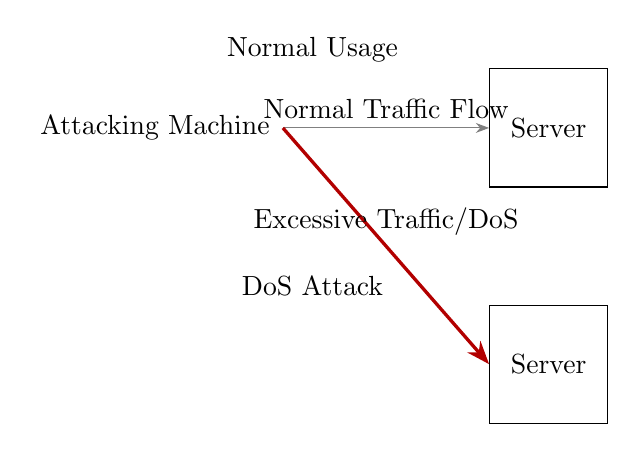
\begin{tikzpicture}[
    >=Stealth,
    comp/.style={rectangle, draw, minimum size=1.5cm},
    flow/.style={->, very thick, red!70!black}
]
\node (Server) at (3, 0) [comp] {Server};
\node (A) at (-2, 0) [draw=none, text width=3cm, align=center] {Attacking Machine};

% Normal Flow
\draw[->, gray] (A.east) -- node[above, black] {Normal Traffic Flow} (Server.west);
\node at (0, 1) [draw=none] {Normal Usage};

% DoS Flow
\node (ServerD) at (3, -3) [comp] {Server};
\draw[->, red!70!black, very thick] (A.east) -- node[above, black] {Excessive Traffic/DoS} (ServerD.west);
\node at (0, -2) [draw=none] {DoS Attack};
\end{tikzpicture}

\subsection{Distributed Denial of Service (DDoS)}
\begin{itemize}
    \item Variation of a DoS attack.
    \item Launched from multiple clients (bots/zombies) controlled by a central controller.
    \item More difficult to track due to the use of \textbf{zombie machines}.
\end{itemize}

\subsection{SYN Flood}
\begin{itemize}
    \item Takes advantage of the TCP handshake process (SYN, SYN-ACK, ACK). The attacking machine sends many SYN requests but never completes the ACK step, exhausting the server's resources.
    \item Mitigation measures:
    \begin{itemize}
        \item Micro Blocks
        \item Bandwidth Throttling
        \item \textbf{SYN Cookies}
        \item \textbf{RST Cookies}
        \item Stack Tweaking
    \end{itemize}
\end{itemize}

\subsubsection{SYN Flood Handshake Comparison}
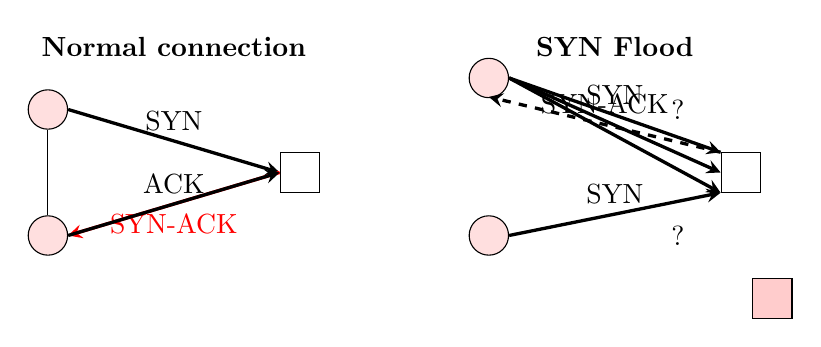
\begin{tikzpicture}[>=Stealth, scale=0.8]
\tikzset{
    host/.style={rectangle, draw, minimum width=0.5cm, minimum height=0.5cm},
    person/.style={circle, draw, fill=pink!50, minimum size=0.5cm},
    line/.style={->, >=stealth, very thick}
}

% --- Normal Connection (Left Side) ---
\node at (0, 5) [font=\bfseries] {Normal connection};
\node (P1) at (-2, 4) [person] {};
\node (P2) at (-2, 2) [person] {};
\node (S) at (2, 3) [host] {};

\draw (P1.south) -- (P2.north); % P1 above P2
\draw[line] (P1.east) -- (S.west) node[midway, above] {SYN};
\draw[line, red] (S.west) -- (P2.east) node[midway, below] {SYN-ACK};
\draw[line] (P2.east) -- (S.west) node[midway, above] {ACK};

% --- SYN Flood (Right Side) ---
\node at (7, 5) [font=\bfseries] {SYN Flood};
\node (PA) at (5, 4.5) [person] {};
\node (PB) at (5, 2) [person] {};
\node (SC) at (9, 3) [host] {};
\node (Overwhelmed) at (9.5, 1) [host, fill=red!20] {};

% Requests
\draw[line] (PA.east) -- (SC.north west) node[midway, above] {SYN};
\draw[line] (PA.east) -- (SC.west);
\draw[line] (PA.east) -- (SC.south west);

% Responses
\draw[line, dashed] (SC.north west) -- (5, 4.2) node[midway, above] {SYN-ACK};

% Unanswered request (PB)
\draw[line] (PB.east) -- (SC.south west) node[midway, above] {SYN};
\node at (8, 4) {?}; % Query response failed
\node at (8, 2) {?};

\end{tikzpicture}

\subsection{Smurf Attack}
\begin{itemize}
    \item A popular DoS attack that utilizes the \textbf{ICMP packet} to execute the attack.
    \item Attacker spoofs the target's IP address and sends ICMP echo requests to the broadcast address of an amplifying network. All hosts in the amplifying network reply to the spoofed target IP, flooding it.
\end{itemize}

\subsection{Ping of Death (PoD)}
\begin{itemize}
    \item Attacks machines that cannot handle oversized packets ($> 65,535$ bytes).
    \item Modern operating systems automatically drop oversized packets.
    \item Mitigation: Ensure systems are patched and up to date.
\end{itemize}

\subsection{UDP Flood and ICMP Flood}
\begin{itemize}
    \item \textbf{UDP Flood}: Variation of PoD that targets open ports. Faster due to no acknowledgments required. Sends packets to random ports, potentially shutting down the target.
    \item \textbf{ICMP Flood}: Another name for the ping flood.
\end{itemize}

\subsection{Distributed Reflection DoS (DRDoS)}
\begin{itemize}
    \item \textbf{DRDoS}: Uses intermediate routers (reflection points) to execute the DoS attack.
    \item Routers do not have to be compromised to execute the attack.
    \item Mitigation: Configure routers to not forward broadcast packets.
\end{itemize}

\section{Malware and Buffer Overflows}

\subsection{Buffer Overflow Attacks}
\begin{itemize}
    \item Occurs when input data exceeds the size of the memory buffer allocated to it, leading to the overflow data overwriting adjacent memory locations.
    \item This can allow attackers to inject malicious code (like script viruses).
\item Mitigation: Bounds checking in programming languages and modern OS security features.
\end{itemize}

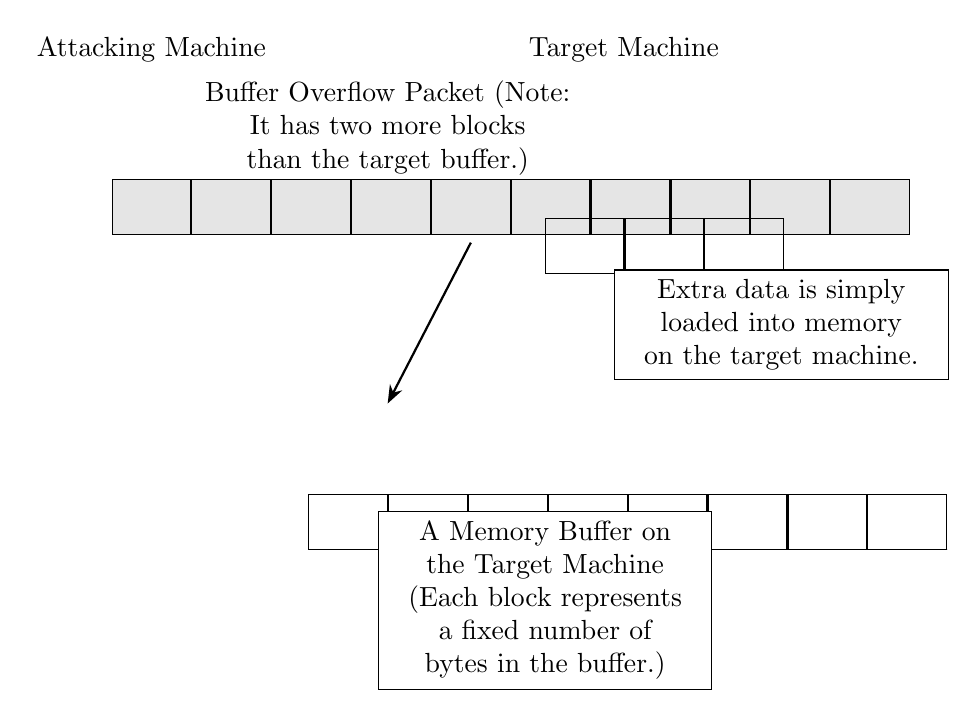
\begin{tikzpicture}[
    >=Stealth,
    block/.style={draw, minimum width=1cm, minimum height=0.7cm},
    data/.style={draw, minimum width=1cm, minimum height=0.7cm, fill=gray!20}
]

\node (Attacker) at (0, 7) [draw=none] {Attacking Machine};
\node (Target) at (6, 7) [draw=none] {Target Machine};

\node (PLabel) at (3, 6) [draw=none, text width=5cm, align=center] {Buffer Overflow Packet (Note: It has two more blocks than the target buffer.)};

\node (D1) at (0, 5) [data] {};
\node (D2) [right=0pt of D1, data] {};
\node (D3) [right=0pt of D2, data] {};
\node (D4) [right=0pt of D3, data] {};
\node (D5) [right=0pt of D4, data] {};
\node (D6) [right=0pt of D5, data] {};
\node (D7) [right=0pt of D6, data] {};
\node (D8) [right=0pt of D7, data] {};
\node (D9) [right=0pt of D8, data] {};
\node (D10) [right=0pt of D9, data] {};

\draw[->, thick] ($(D5.south)+(0, -0.1)$) -- (3, 2.5);

\node (T1) at (2.5, 1) [block] {};
\node (T2) [right=0pt of T1, block] {};
\node (T3) [right=0pt of T2, block] {};
\node (T4) [right=0pt of T3, block] {};
\node (T5) [right=0pt of T4, block] {};
\node (T6) [right=0pt of T5, block] {};
\node (T7) [right=0pt of T6, block] {};
\node (T8) [right=0pt of T7, block] {};

\draw (T1.south west) rectangle (T8.south east);
\node at (5, 0) [draw, fill=white, text width=4cm, align=center] {A Memory Buffer on the Target Machine (Each block represents a fixed number of bytes in the buffer.)};

\node (E1) at (5.5, 4.5) [block] {};
\node (E2) [right=0pt of E1, block] {};
\node (E3) [right=0pt of E2, block] {};
\node at (8, 3.5) [draw, fill=white, text width=4cm, align=center] {Extra data is simply loaded into memory on the target machine.};

\end{tikzpicture}

\subsection{Malware Definitions}
\begin{itemize}
    \item \textbf{Virus}: Malware that replicates when executed.
    \begin{itemize}
        \item Requires human interaction to spread.
        \item Spreads by reading email address books or attaching to existing email software.
    \end{itemize}
    \item \textbf{Worm}: Malware that can spread without human interaction.
    \begin{itemize}
        \item Spreads by scanning computers for network connections and copying itself to machines with write access.
    \end{itemize}
    \item \textbf{Logic Bomb}: A set of instructions secretly incorporated into a program that are carried out only if a particular condition is satisfied (e.g., date, specific action).
    \item \textbf{Backdoor}: Covert method of bypassing normal authentication or encryption.
    \item \textbf{Trojan Horse Attacks}: A program that looks benign but has malicious intent.
    \begin{itemize}
        \item Actions include: downloading harmful software, installing keyloggers/spyware, deleting files, or opening a backdoor.
        \item Symptoms: Home page changes, unexpected changes to passwords/accounts/screen savers/settings, devices working on their own (e.g., CD door).
    \end{itemize}
    \item \textbf{Ransomware}: A malware payload that locks down the user’s files until they pay a ransom.
\end{itemize}

\section{Risk Calculation}

\subsection{Single Loss Expectancy (SLE)}
Calculates the impact a single loss will cause.
\begin{itemize}
    \item \textbf{Asset value (AV)}: Current value of the asset.
    \item \textbf{Exposure factor (EF)}: Percentage of the asset’s value that will be lost (0.0 to 1.0).
    \item Formula:
    $$ \textbf{SLE} = \textbf{AV} \times \textbf{EF} $$
    \item Example: A one-year-old laptop originally costing \$800 with 10\% depreciation has an AV of \$720. If EF is 0.9, $\text{SLE} = 720 \times 0.9 = \$648$. (Note: Slide uses 800 AV and 0.9 EF for \$720 result, which implies 0\% depreciation was applied for the formula step.)
\end{itemize}

\subsection{Annualized Loss Expectancy (ALE)}
Calculates how much loss you can expect from a particular issue in a year.
\begin{itemize}
    \item \textbf{Annual Rate of Occurrence (ARO)}: How often the event is expected to occur in one year.
    \item Formula:
    $$ \textbf{ALE} = \textbf{SLE} \times \textbf{ARO} $$
    \item Example: If $\text{SLE} = 720$ and you estimate losing 6 laptops a year ($\text{ARO} = 6$), $\text{ALE} = 720 \times 6 = \$4320$.
\end{itemize}

\subsection{Evaluating the Security Risk}
Risk is calculated based on three factors, each scored 1 to 10:
\begin{itemize}
    \item \textbf{Attractiveness (A)} to hackers.
    \item \textbf{Information (I)} content (Nature of information).
    \item \textbf{Security (S)} (Level of security measures in place).
    \item Formula:
    $$ (\textbf{A} + \textbf{I}) - \textbf{S} = \textbf{Rating (R)} $$
    \item The lower the rating, the more secure the system.
\end{itemize}

\section{The Six P’s of Assessment}
\begin{enumerate}
    \item Patches
    \item Ports
    \item Protect
    \item Physical
    \item Probe
    \item Policies
\end{enumerate}

\subsection{(1) Patches}
\begin{itemize}
    \item \textbf{Patch policy}: Must be written and followed.
    \item \textbf{Applying patches}: Must check all applications. Should be the first step in assessing the system.
    \item Automated patch systems examples: Windows Update, HFNetChkPro, ZenWorks Patch Management, McAfee ePolicy Orchestrator.
\end{itemize}

\subsection{(2) Ports}
\begin{itemize}
    \item Common virus attacks come through specific ports.
    \item Action: Close all unused ports to reduce vulnerability.
\end{itemize}

\subsection{(3) Protect}
Ensure the following protection measures are in place and functioning:
\begin{itemize}
    \item Firewall
    \item Antivirus protection
    \item Antispyware
    \item \textbf{IDS} (Intrusion Detection System)
    \item Proxy server or \textbf{NAT} (Network Address Translation)
    \item Data transmission encryption
\end{itemize}

\subsection{(4) Physical}
Control access to:
\begin{itemize}
    \item Server rooms
    \item Workstations
    \item Miscellaneous equipment
    \item Data backup media
\end{itemize}
Additional Physical Security Strategies: Biometric locks, logging/escorting visitors, inspecting bags, prohibiting portable recording devices, logging printing and copying.

\subsection{(5) Probe}
Methods for discovering vulnerabilities:
\begin{itemize}
    \item \textbf{Port scanning}: Scan well-known ports to see which are open.
    \item \textbf{Enumerating}: Try to determine what is on the target network (accounts, shares, printers).
    \item \textbf{Vulnerability assessment}: Use tools or manual methods to seek out known vulnerabilities.
\end{itemize}
Vulnerability Lists:
\begin{itemize}
    \item \textbf{Common Vulnerabilities and Exposures (CVE)}: Maintained by the Mitre Corporation.
    \item \textbf{National Institute of Standards and Technology (NIST)}: Uses the CVE format.
    \item \textbf{Open Web Application Security Project (OWASP)}: The standard for web application security; publishes the Top 10 List.
\end{itemize}

\subsection{(6) Policies - Security Documentation}

\subsubsection{McCumber Cube (Security Framework)}
Defines three dimensions of security:
\begin{itemize}
    \item \textbf{Goals (CIA triad)}: Confidentiality, Integrity, Availability.
    \item \textbf{Information States}: Storage, Transmission, Processing.
    \item \textbf{Safeguards}: Policy and Practices, Human Factors, Technology.
\end{itemize}

\subsubsection{Required Documentation}
\begin{itemize}
    \item \textbf{Physical security documentation}: List security in place, document location of every device, key lists for locked rooms, copies of entry logs.
    \item \textbf{Policy and personnel documentation}: All policies must be filed, revisions documented, signed copies of agreements on awareness, list of personnel with access rights.
    \item \textbf{Probe documents}: Internal/external audit results, follow-up reports on flaws, documentation of security incidents and corrections.
    \item \textbf{Network protection documents}: Details of:
    \begin{itemize}
        \item Firewall use and configuration.
        \item IDS use and configuration.
        \item Antivirus/antispyware used.
        \item Honeypots in use.
        \item Individual machine security measures.
    \end{itemize}
\end{itemize}

\section{Security Roles and Wireless Attacks}

\subsection{Types of Hackers}
\begin{itemize}
    \item A \textbf{white hat hacker} (penetration tester) hacks with permission of the system owners (i.e., they are \textbf{AUTHORIZED} to simulate a cyber attack).
    \item A \textbf{black hat hacker} (cracker) gains access to cause harm.
    \item A \textbf{gray hat hacker} is normally law-abiding but may venture into illegal activities.
\end{itemize}

\subsection{Evil Twin Attack}
\begin{itemize}
    \item \textbf{Evil Twin}: A fraudulent Wi-Fi access point that appears legitimate but is set up to eavesdrop on wireless communications.
    \item It is the wireless LAN equivalent of a phishing scam.
\end{itemize}

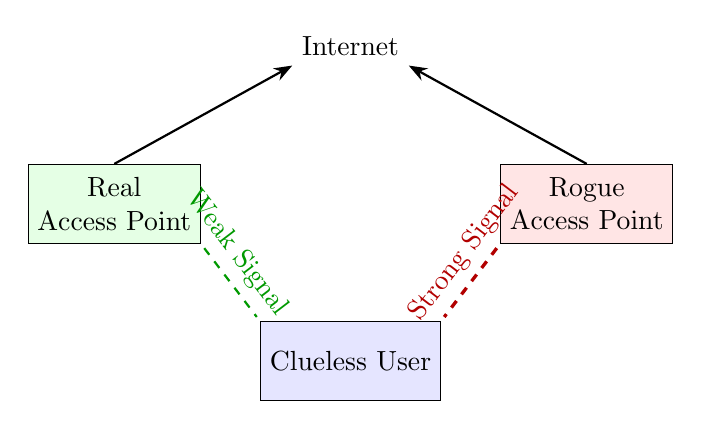
\begin{tikzpicture}[
    >=Stealth,
    node distance=2.5cm,
    ap/.style={rectangle, draw, minimum width=1.5cm, minimum height=1cm, align=center, fill=gray!10},
    user/.style={rectangle, draw, minimum width=1.5cm, minimum height=1cm, fill=blue!10},
    signal/.style={dashed, thick, shorten >=2pt, shorten <=2pt},
    connection/.style={->, thick},
]

\node (Internet) at (3, 4) [draw=none] {Internet};

% Access Points
\node (RealAP) at (0, 2) [ap, fill=green!10] {Real \\ Access Point};
\node (RogueAP) at (6, 2) [ap, fill=red!10] {Rogue \\ Access Point};

% User
\node (CluelessUser) at (3, 0) [user] {Clueless User};

% Connections to Internet
\draw[connection] (RealAP.north) -- (Internet.south west);
\draw[connection] (RogueAP.north) -- (Internet.south east);

% Signals to User
\draw[signal, green!60!black] (RealAP.south east) -- node[above, sloped, near end, pos=0.3] {Weak Signal} (CluelessUser.north west);
\draw[signal, red!70!black, very thick] (RogueAP.south west) -- node[above, sloped, near end, pos=0.3] {Strong Signal} (CluelessUser.north east);

\end{tikzpicture}

\end{document}
